%Brechungsindex
Licht bewegt sich im Vakuum mit der bekannten Vakuum-Lichtgeschwindigkeit $c_{\text{0}}$.
In Medien kommt es zu einer Wechselwirkung des Lichts mit dem Material und die Ausbreitungsgeschwindigkeit $c$ verringert sich.
Trifft eine Lichtwelle in einem Winkel auf eine Grenzfläche zwischen zwei Medien, dann kommt es zur Lichtbrechung, also einer Änderung der Ausbreitungsrichtung.
An dieser Grenzfläche ist die Richtungsänderung abhängig von den Lichtgeschwindigkeiten in den jeweiligen Medien.
Dies lässt sich im Brechungsindex $n$ zusammenfassen:
\begin{align}
   n=\frac{c_{\text{1}}}{c_{\text{2}}}.
   \label{eqn:brechung}
\end{align}
%Huygens-Prinzip
\\Das Huygens'sche Prinzip sagt nun, dass jeder einzelne Oszillator einer Welle der Ausgangspunkt einer neuen Welle sein kann.
Beim schrägen Auftreffen auf eine Grenzfläche kommen nun mehrere Oszillatoren leicht zeitversetzt an der Grenzfläche an (Abb. \ref{fig:huygens}).
\begin{figure}[h!]
  \centering
  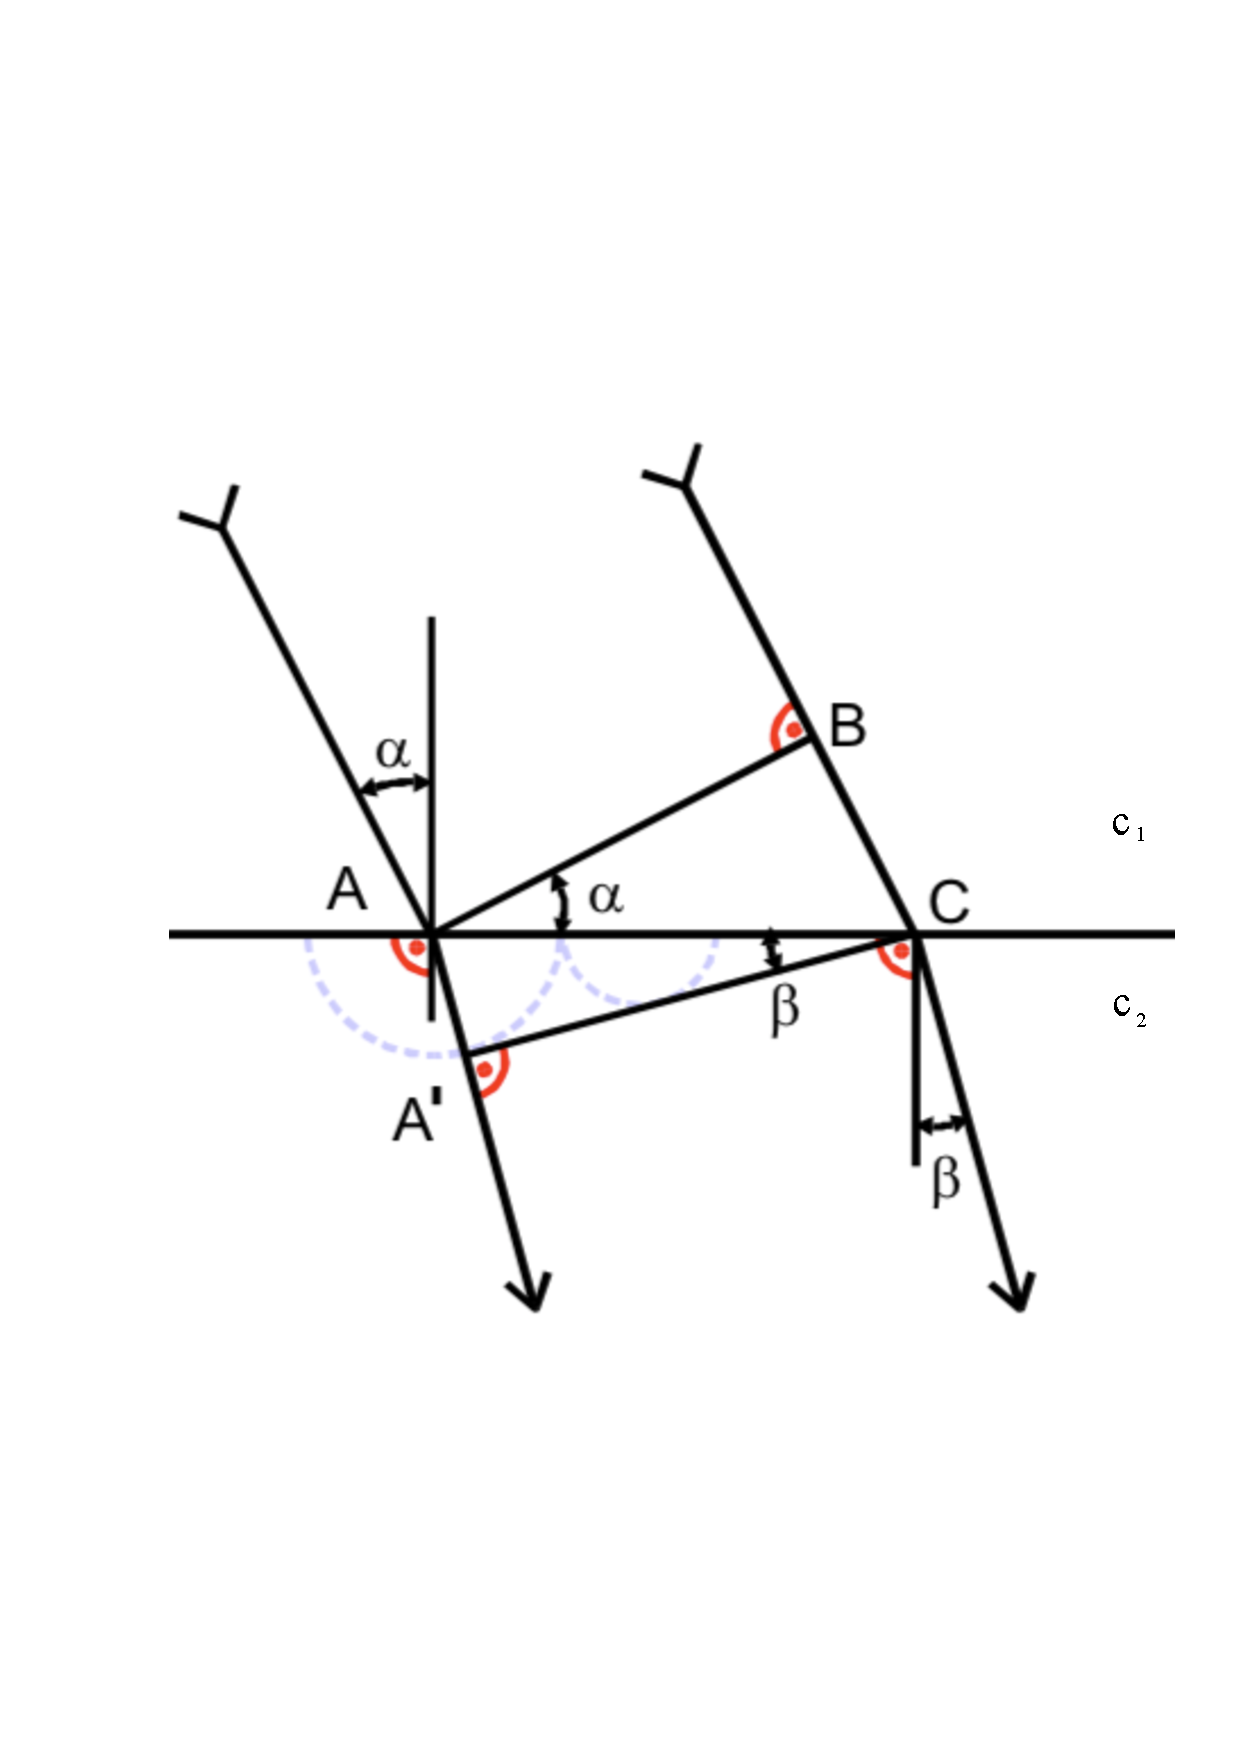
\includegraphics[width=0.8\textwidth]{huygens.pdf}
  \caption{Lichtbrechung durch das Huygens'sche Prinzip \cite{1}}
  \label{fig:huygens}
\end{figure}
Im ersten Medium benötigt die Welle die Zeit $T$ um die Stecke $\overline{BC}$ zurückzulegen:
\begin{align*}
  \overline{BC}= c_{\text{1}} T.
\end{align*}
Außerdem lässt sich die Winkelbeziehung
\begin{align*}
  \overline{BC} =\overline{AC} \sin{(\alpha)} = c_{\text{1}} T \Leftrightarrow  c_{\text{1}} = \sin{(\alpha)} \frac{\overline{AC}}{T}
\end{align*}
aufstellen.
Wenn die Welle im Punkt C angekommen ist, ist im Punkt A bereits eine neue Welle im zweiten Medium entstanden und hat sich bis zum Punkt A' fortbewegt.
Für die Strecke $\overline{A A'}$ im zweiten Medium braucht die Welle ebenfalls die Zeit $T$:
\begin{align*}
  \overline{AA'}= c_{\text{2}} T.
\end{align*}
Erneut lässt sich eine Winkelbeziehung aufstellen:
\begin{align*}
  \overline{AA'}= \overline{AC} \sin{(\beta)} = c_{\text{2}} T \Leftrightarrow c_{\text{2}} = \sin{(\beta)} \frac{\overline{AC}}{T}.
\end{align*}
Das Verhältnis beider Lichtgeschwindigkeiten beschreibt nach Gleichung \eqref{eqn:brechung} den Brechungsindex $n$:
\begin{align}
  n=\frac{c_{\text{1}}}{c_{\text{2}}} = \frac{\sin{(\alpha)}}{\sin{(\beta)}}.
  \label{eqn:brechungsindex}
\end{align}
%Dispersion
\\Der Brechungsindex $n$ ist aber auch von der Energie $E$ des Lichts abhängig.
Die Energie lässt sich mit dem Planck'schen Wirkungsquantum $h$ und der Frequenz $\nu$ als
\begin{align*}
  E= h \nu = \frac{h c_{\text{0}}}{\lambda}
\end{align*}
schreiben.
Mit der Beziehung $c_{\text{0}}=\nu/\lambda$ wird die Wellenlängenabhängigkeit des Energie deutlich.
Damit ist der Brechungsindex $n$ abhängig von der Wellenlänge des Lichts $\lambda$: $n(\lambda)$.
Diese Abhängigkeit wird Dispersion genannt.
Die Dispersion lässt sich allgemeiner über die Frequenzabhängigkeit der Ausbreitungsgeschwindigkeit $c(\nu)$ definieren.
%Dispersionsgleichung
\\Wie bereits anfänglich beschrieben, gibt es eine Wechselwirkung des Lichts mit der Materie beim Durchlaufen eines Mediums.
Diese Wechselwirkung wird nun genauer betrachtet um die Dispersionsgleichung herzuleiten.
Das Licht setzt sich aus einem elektrischen und einem magnetischen Feld zusammen.
Fällt also eine Lichtwelle durch ein Material, wirkt auf das Material die resultierende Kraft $F_{\text{E}}$ durch das elektrische Feld $E$:
\begin{align*}
  \vec{F_{\text{E}}}= q E = q \vec{E_{\text{0}}} e^{i \omega t}.
\end{align*}
Allgemein erfährt ein Teilchen im Medium bei der Beschwleunigung $a$ die Kraft $F_{\text{a}}$:
\begin{align*}
  F_{\text{a}}= m a = m \frac{d^2 x}{d t^2}.
\end{align*}
Auf dasselbe Teilchen wirkt eine rücktreibende Kraft $F_{\text{rücktreibend}}$:
\begin{align*}
  F_{\text{rücktreibend}}= b x.
\end{align*}
Außerdem wirkt die Reibungskraft $F_{\text{Reibung}}$:
\begin{align*}
  F_{\text{Reibung}}= f \frac{d x}{d t}.
\end{align*}
Die Summe der Kräfte dann zur Bewegungsgleichung:
\begin{align}
  m \frac{d^2 x}{d t^2} + f \frac{d x}{d t} + b x = q \vec{E_{\text{0}}} e^{i \omega t}.
  \label{eqn:disp1}
\end{align}
Die Bewegungsgleichung lässt sich auch durch die Polarisation ausdrücken.
Die Polarisation beschreibt die Verschiebung der Teilchen in der Materie durch das magnetische Feld der Lichtwelle.
Die Polarisation ergibt sich dann als Summe $P$ aller Dipolmomente $d=q x$:
\begin{align*}
  P= \sum N_{\text{h}} q_{\text{h}} x_{\text{h}}.
\end{align*}
Damit lässt sich die Bewegungsgleichung \eqref{eqn:disp1} umschreiben zu
\begin{align*}
  \frac{d^2 P}{d t^2}+\frac{f}{m} \frac{d P}{d t}+ \frac{b}{m}P = \frac{N q^2 E_{\text{0}}}{m} e^{i \omega t}.
\end{align*}
Die Lösung der obigen Dispersionsgleichung lautet
\begin{align*}
  P= \frac{N q^2}{m\left(\omega^2_{\text{h}}-\omega^2+i\frac{f}{m}\omega \right)} E_{\text{0}} e^{i \omega t}.
\end{align*}
Dies beschreibt die Polariation pro Teilchen.
Die gesamte Polariation ist also die Summe aller Polarisationen.
Wird die Polarisation $P$ durch die dielektrische Verschiebung $P=(\epsilon -1)\epsilon_{\text{0}}\vec{E}$ ersetzt, lässt sich mithilfe der Maxwell'schen Relation $n^2=\epsilon$ schreiben:
\begin{align*}
  n^2 = \epsilon = 1+\sum_{\text{h}} \frac{N_{\text{h}} q_{\text{h}}^2}{m \epsilon_{\text{0}}\left(\omega^2_{\text{h}}-\omega^2+i\frac{f_{\text{h}}}{m_{\text{h}}}\omega \right)}.
\end{align*}
Es wird angenommen, dass außerhalb der Resonanzbereiche gemessen wird: $n^2 k=0$.
Dadurch folgt mit $\omega=\frac{\nu}{2 \pi}=\frac{c}{2 \pi \lambda}$:
\begin{align*}
                  &n^2(\omega)=   & 1+\sum_{\text{h}} \frac{N_{\text{h}} q_{\text{h}}^2}{m \epsilon_{\text{0}}\left(\omega^2-\omega^2_{\text{h}} \right)}\\
  \Leftrightarrow &n^2(\lambda)=  & 1+\sum_{\text{h}} \frac{N_{\text{h}} q_{\text{h}}^2 \lambda^2 \lambda_{\text{h}}^2 }{ 4 \pi^2 c^2 m \epsilon_{\text{0}}\left(\lambda^2-\lambda^2_{\text{h}} \right)}.
\end{align*}
Die Entwicklung der Potenzen ergibt für $\lambda_{\text{1}} \ll \lambda$ und für $\lambda \ll \lambda_{\text{1}}$ unterschiedliche Gleichungen.
Für $\lambda_{\text{1}} \ll \lambda$ (Abb. \ref{fig:größer}) ergibt sich:
\begin{align}
  n^2(\lambda)  &=   1+ \frac{N_{\text{1}} q_{\text{1}}^2 \lambda_{\text{1}}^2}{4 \pi^2 c^2 \epsilon_{\text{0}} m_{\text{1}}} \left(1 + \left( \frac{\lambda_{\text{1}}}{\lambda} \right)^2 + \left( \frac{\lambda_{\text{1}}}{\lambda} \right)^2 + ...\right)\\
                &=   A_{\text{0}} + \frac{A_{\text{2}}}{\lambda^2} + \frac{A_{\text{4}}}{\lambda^4} + ...
  \label{eqn:größer}
\end{align}
\begin{figure}[h!]
  \centering
  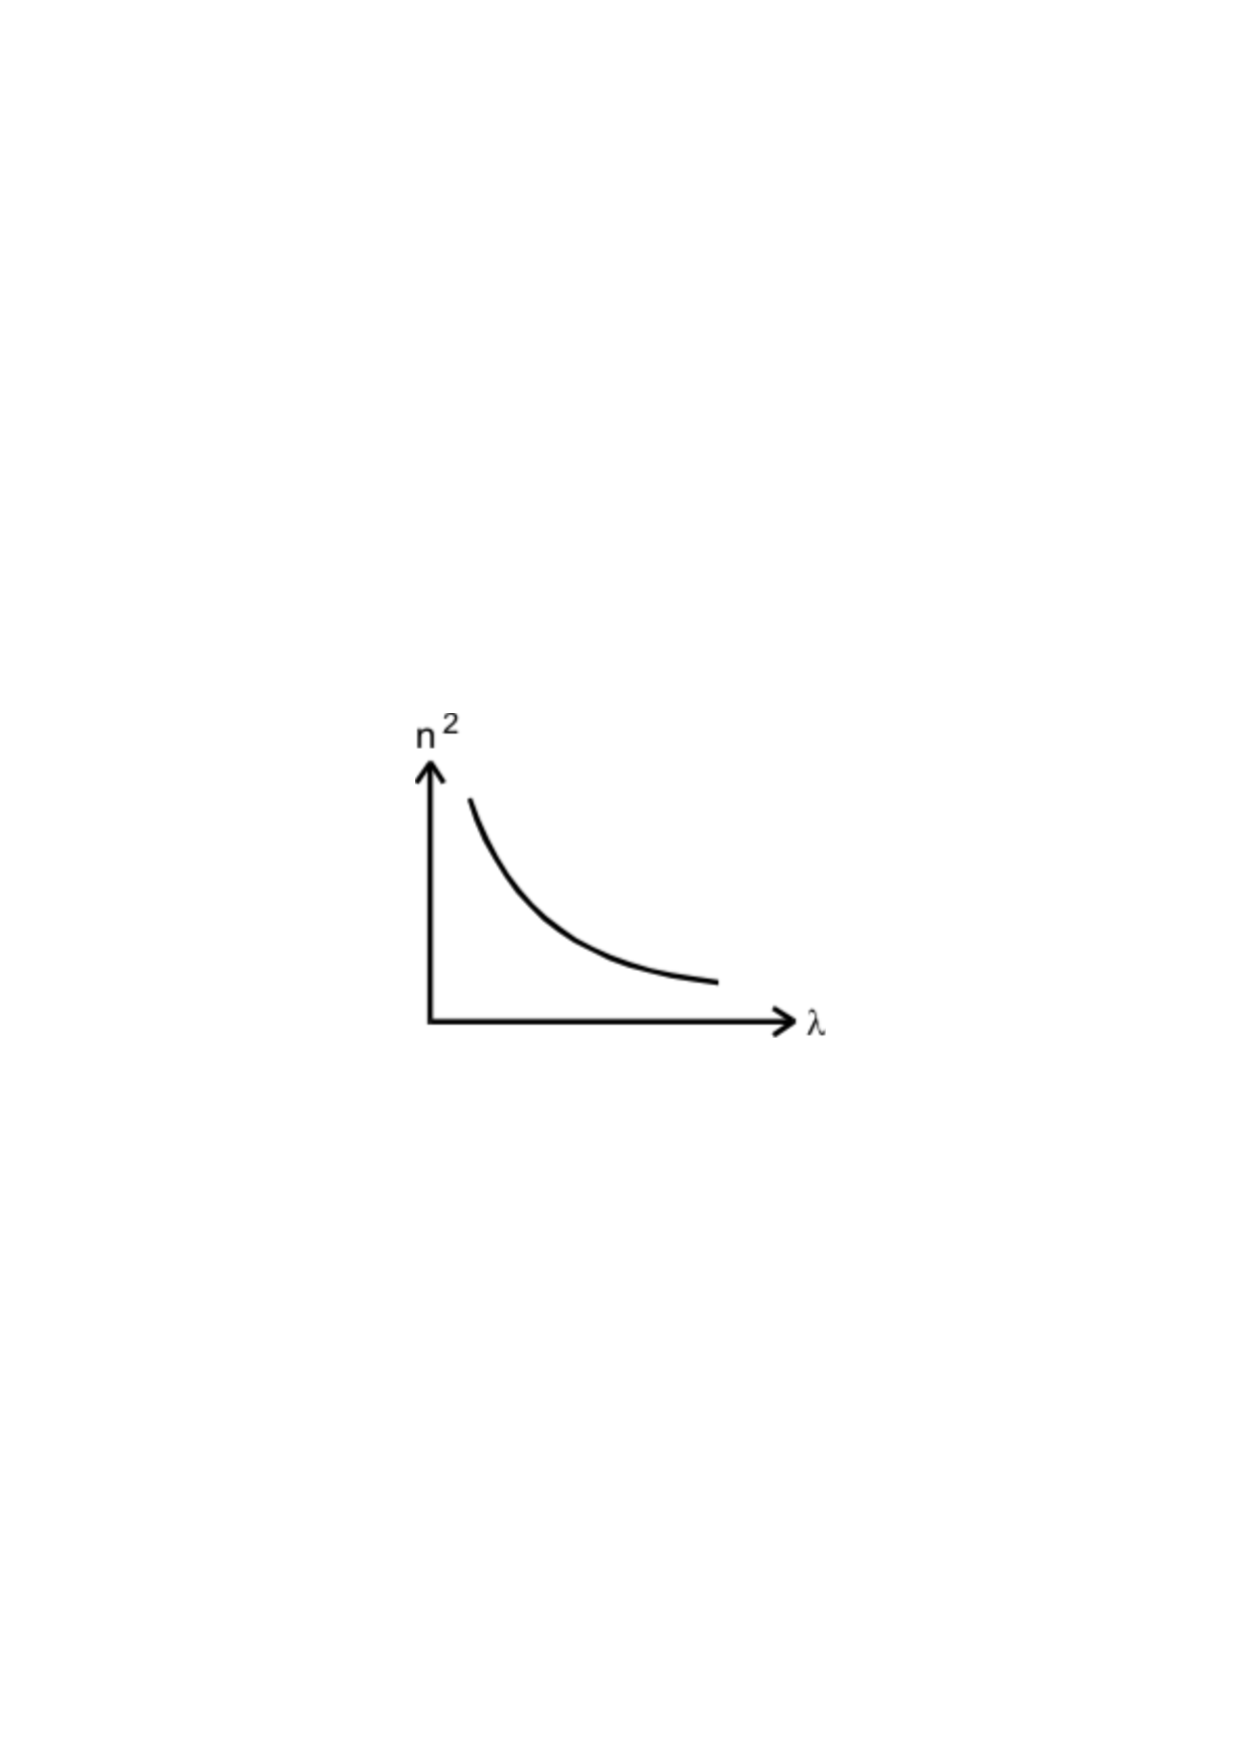
\includegraphics[width=0.4\textwidth]{größer.pdf}
  \caption{Kurvenverlauf für $\lambda_{\text{1}} \ll \lambda$ \cite{1}}
  \label{fig:größer}
\end{figure}
\FloatBarrier
Für $\lambda \ll \lambda_{\text{1}}$ (Abb. \ref{fig:kleiner}) gilt:
\begin{align}
  n^2(\lambda)=1 - A_{\text{2}} \lambda^2 - A_{\text{4}} \lambda^4 - ...
  \label{eqn:kleiner}
\end{align}
\begin{figure}[h!]
  \centering
  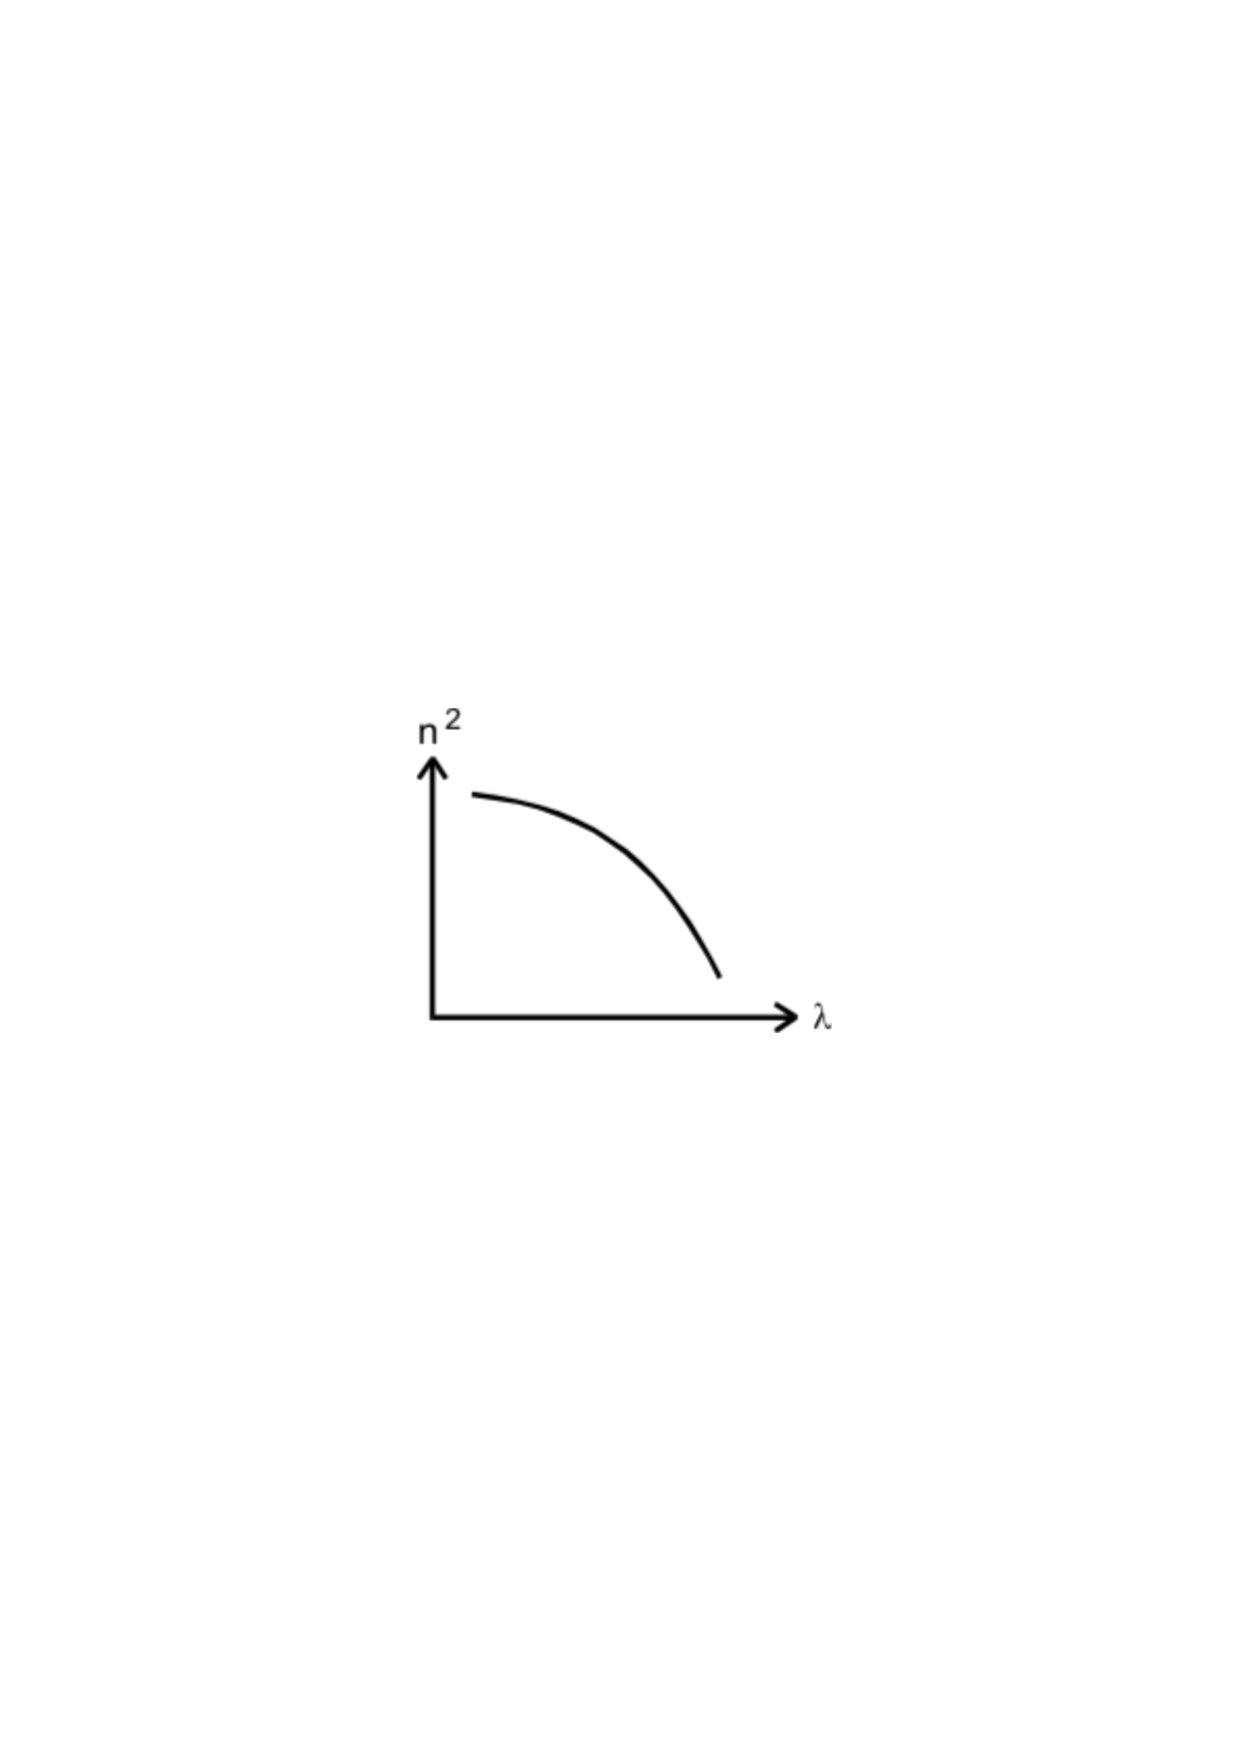
\includegraphics[width=0.4\textwidth]{kleiner.pdf}
  \caption{Kurvenverlauf für $\lambda \ll \lambda_{\text{1}}$ \cite{1}}
  \label{fig:kleiner}
\end{figure}
Das monoton fallende Verhalten der Kurven beschreibt die normale Dispersion.
In der Nähe der Resonanzfrequenz ist auch ein monoton steigendes Verhalten möglich.
Dies wird anormale Dispersion genannt.
%Prismen
\\Betrachtet wird nun der symmetrische Strahlengang durch ein Glasprisma:
\begin{figure}[h!]
  \centering
  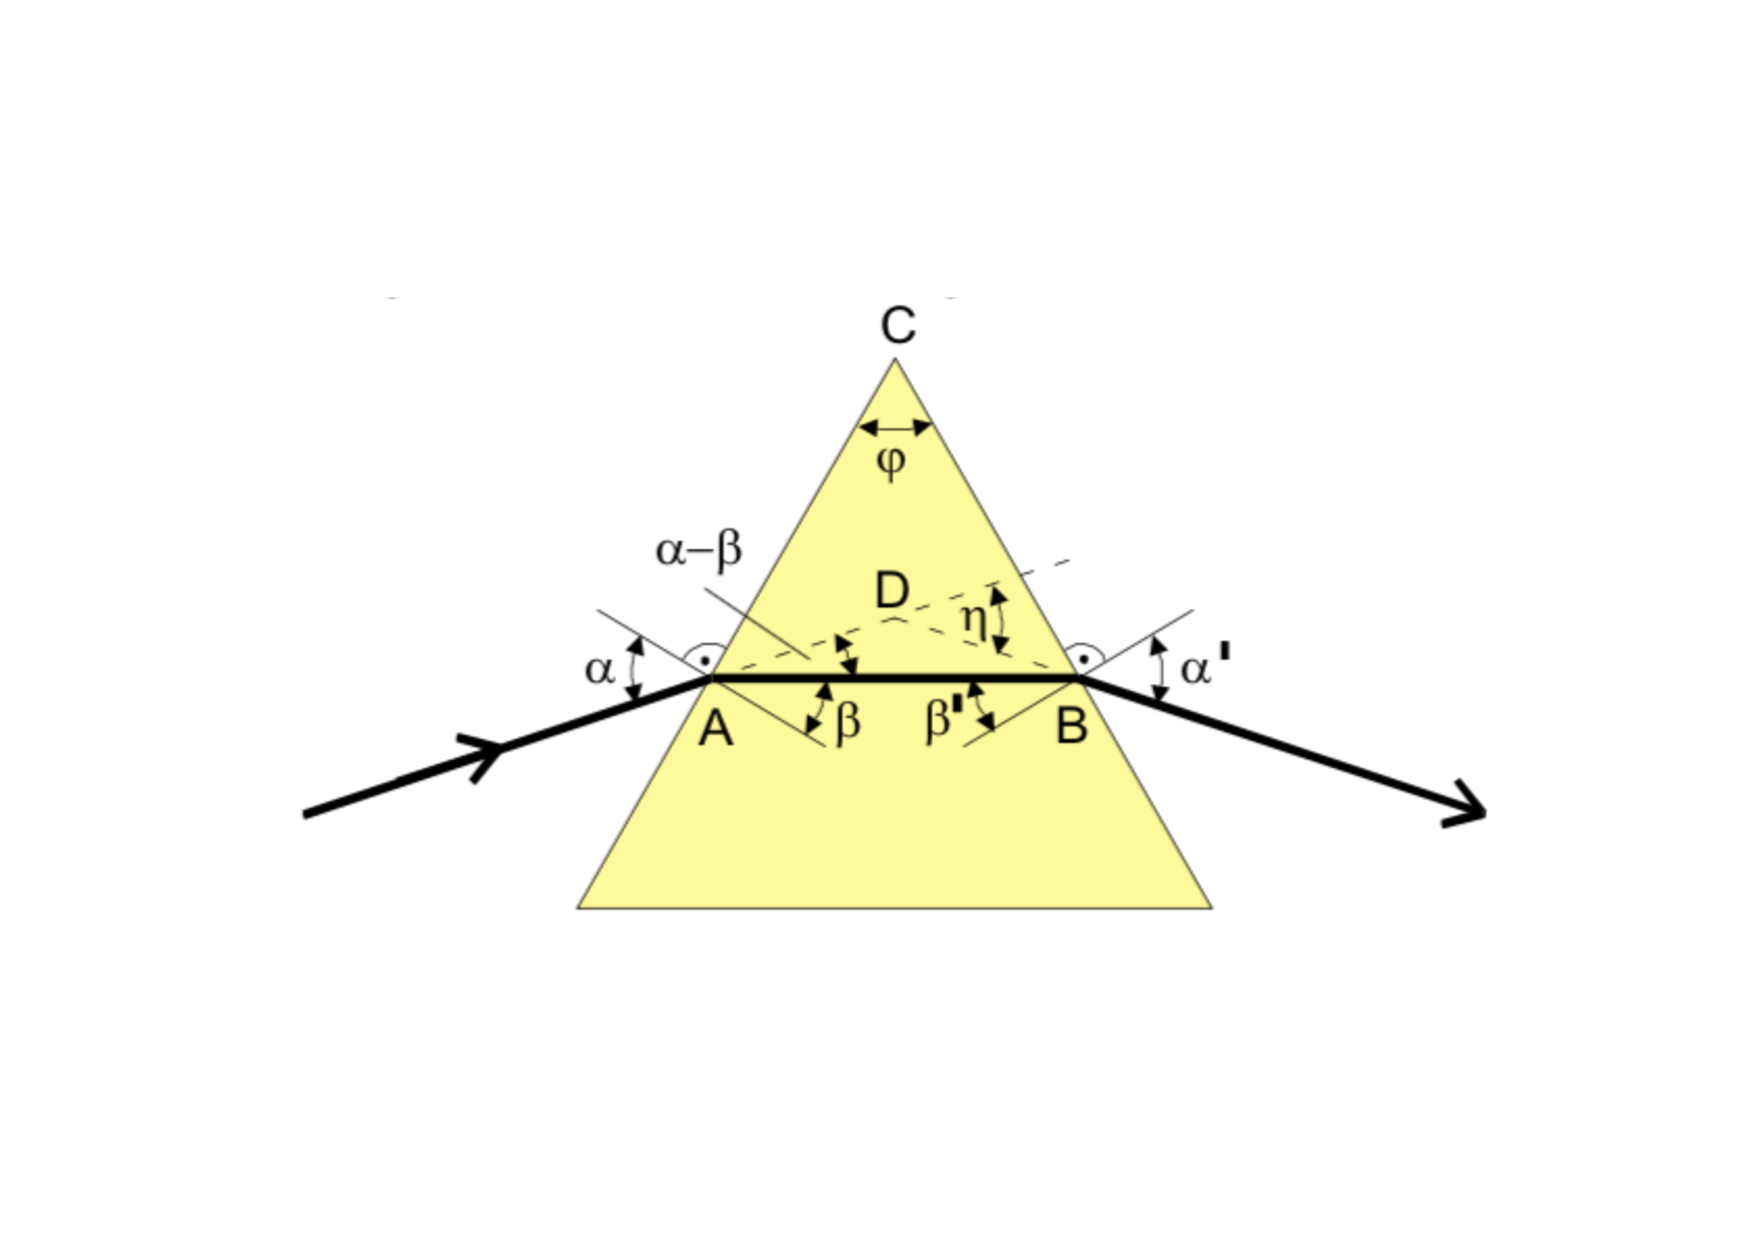
\includegraphics[width=0.8\textwidth]{prisma.pdf}
  \caption{Strahlengang im Prisma \cite{1}}
  \label{fig:prisma}
\end{figure}
Die Strahlen werden zwei Mal gebrochen.
Aus den Winkelbeziehungen folgt, dass
\begin{align*}
  \beta=\frac{\varphi}{2}
\end{align*}
ist und dass
\begin{align*}
  \eta= 2(\alpha - \beta) \Leftrightarrow \alpha = \frac{\eta}{2}+\beta = \frac{\eta+\varphi}{2}
\end{align*}
gilt.
Mit Gleichung \eqref{eqn:brechungsindex} ergibt sich
\begin{align}
  n= \frac{ \sin{ \left( \frac{\eta+\varphi}{2} \right)} }{ \sin{ \left( \frac{\varphi}{2} \right)} }.
\end{align}


\FloatBarrier
